\documentclass[11pt,a4paper]{article}
\usepackage[utf8]{inputenc}
\usepackage[ngerman]{babel}
\usepackage{hyperref}
\usepackage{graphicx} 
\usepackage{listings}
\usepackage{concmath}
\usepackage[T1]{fontenc}
\usepackage{amsmath}

\author{Moritz Basel, Samuel Metzler, Dominik Weissenseel}
\title{Interne Mitfahrgelegenheit}
\date{\today{}}
\begin{document}
\normalfont


\maketitle{}
\tableofcontents{}

\section{Einführung}
\subsection{Zweck des Dokuments}
In diesem Dokument wird der Umfang und die Funktionalität des Systems (``die Software'') ``Interne Mitfahrgelegenheit'' spezifiziert, sowie deren Architektur umrissen.
\subsection{Zweck der Software}
Die Software stellt ein System zur automatischen Verteilung von Mitfahrern auf Autos zur Verfügung. Zu festgesetzten Terminen stellen Teilnehmer Autos zur Verfügung oder teilen ihren Wunsch mitgenommen zu werden mit.
\subsection{Zielgruppe}
Die Software richtet sich an mittlere bis große Organisationen, die oft oder regelmäßig Fahrten von einem definiertem Startort zu verschiedenen Zielorten unternimmt und dabei auf private Autos der Teilnehmer setzt.

\section{Beschreibung}
\subsection{Funktionen}
Die Software stellt alle Funktionen eines webbasierten Login-Dienstes sowie die zugehörige administrative Funktionalität  bereit.
\subsubsection{Login-Funktionalitäten}
\begin{itemize}
\item Signup - Erstellen von Nutzern
\item Login - Login eines Nutzers
\end{itemize}
\subsubsection{Administrative Funktionalitäten}
\begin{itemize}
\item Delete User - Löschen von Nutzern
\item Diagnostics - Einsehen von Daten zu allen Nutzern und Appointments
\end{itemize}
\subsubsection{Appointments}
Appointments stellen das Herzstück der Software dar. Nutzer bzw. Administratoren erstellen Appointments, die von allen Nutzern eingesehen werden können. Nach der Erstellung existiert ein Zeitrahmen, in dem andere Nutzer sich als MUSS-Fahrer, KANN-Fahrer oder MIT-Fahrer eintragen. In den ersten beiden Fällen geschieht dies zusammen mit einer Kapazitätsangabe.
Am Ende der Frist werden alle Teilnehmer nach logischen Regeln auf die angemeldeten Autos verteilt oder es wird ein Fehlerereignis generiert, wenn nicht genügend Plätze vorhanden sind.
Nach der Fahrt validieren alle aktiven Fahrer ihre Fahrt und das Appointment wird archiviert.
\subsection{MUSS-Kriterien}
\begin{itemize}
\item Klares, per TLS gesichertes System zum Einloggen, zur Übertragung der Daten und zur Persistenz derselben
\item Fähigkeit des Nutzers, Appointments zu erstellen, zu löschen und alle aktiven anzuzeigen
\item Anmelden zu einem bestehendem Appointment um mitgenommen zu werden, garantiert mit dem eigenen Auto zu fahren oder es vom System entscheiden zu lassen
\item Anzeigen der vorläufigen Fahrerverteilung zu einem Appointment
\item Klare Meldung zu unvollständigen Appointments mit Aufforderung der Lösung des Problems durch Menschen (z.B. via Email)
\end{itemize}

\subsection{KANN-Kriterien}
\begin{itemize}
\item Trennung von Organisationen, entweder zum Betrieb als Master-Server mit mehreren Organisationen als Nutzer oder zur Trennung von Suborganisationen
\item Faire Verteilung der KANN-Fahrer, z.b. via Speicherung gefahrener Kilometer oder einfach Zählen aller erfolgter Fahrten
\end{itemize}
\subsection{Abgrenzungskriterien}
\begin{itemize}
\item Die Anwendung wird weder Fahrtengeld berechnen noch regeln.
\item Es wird keine direkte Kommunikation zwischen Teilnehmern eines Appointments unterstützt; die Mitfahrer müssen die Kontaktaufnahme mit den Fahrern selbst selbst initiieren.
\item Die Anwendung wird keine Zwischenhalte oder Treffpunkte fuer ein Appointment bestimmen.
\item Die Fahrtroute wird nicht geplant werden.
\item Die Wohnorte von Nutzern werden nicht verwaltet und nicht bei der Aufteilung der Mitfahrer auf Fahrer berücksichtigt.
\item Die Anwendung wird nicht als öffentlicher Service dienen, sondern von Organisationen, die diese nutzen möchten, selbst gehostet und verwaltet.
\item Es wird kein Feature zur Meldung von unangebrachten Verhalten eines anderen Nutzers geben.
\item Es wird keine Garantie für eine reibungslose Aufteilung der Nutzer geben. Die Anwendung liefert vernünftige Vorschläge, jedoch muss die endgültige Absprache von den Nutzern persönlich erledigt werden.
\end{itemize}

\subsection{Nichtfunktionale Anforderungen}
\begin{itemize}
\item Sämtliche API-Calls finden ausschließlich verschlüsselt via HTTPS/TLS statt.
\item Die Antwortzeit des Systems darf für keine Anfrage zwei (2) Sekunden übersteigen und sollte meistens unter 0.5 Sekunden liegen.
\end{itemize}


\section{User Stories}
\subsection{Erstellung und Anmeldung für Appointments}
\subsection*{Nutzer erstellt ein Appointment}
Der Nutzer gibt Abfahrtszeit, Anmeldungsdeadline, Abfahrtsort und Zielort an. Der Nutzer kann nun auswählen, ob er das Appointment als MUSS-FAHRER, KANN-FAHRER oder MITFAHRER erstellt. Wenn der Nutzer die Rolle MUSS-FAHRER oder KANN-FAHRER wählt, gibt er zusätzlich die maximale Anzahl an Fahrtgästen an, die er in seinem Auto mitnehmen kann. Abschließend bestätigt er seine Angaben und das Appointment wird veröffentlicht.

\subsection*{Nutzer meldet sich bei einem Appointment an}
Der Nutzer ruft die Liste von Appointments auf. Dem Nutzer werden daraufhin eine Liste von aktiven Appointments (bei welchen die Anmeldungsdeadline noch nicht abgelaufen ist) angezeit. Der Nutzer waehlt eines der Appointments aus, und meldet sich als MUSS-FAHRER, KANN-FAHRER oder MITFAHRER an. Wenn der Nutzer die Rolle MUSS-FAHRER oder KANN-FAHRER wählt, gibt er zusätzlich die maximale Anzahl an Fahrtgästen an, die er in seinem Auto mitnehmen kann.

\subsection{Ausnahmebehandlung}
\subsection*{Absage eines Fahrers nach Anmeldungsdeadline}
Der Fahrer ruft die Liste der Appointments auf, an denen er sich beteiligt. Er wählt das Appointment, für welches er seine Teilnahme absagen möchte. Das System benachrichtigt die anderen Fahrer, seine Mitfahrer und versucht die Kollision mit möglichst wenig propagierenden Konsequenzen aufzulösen.

\section{Architektur}
Die Software wird zur Wahrung der Extensionalität strikt zwischen Backend (Server) und Frontend (Client) getrennt. Das Frontend kann z.B. in Form einer Website, einer webbasierten Mobile App (z.B. Cordova) oder einer nativen Mobile App (Android, iOS) vorliegen.
\bigskip\\
Geplant ist eine Andriod-App.
\subsection{REST-Schnittstelle}
Die Spezifikation der REST-API befindet sich in einem separatem Dokument.
Datenaustausch findet via JSON statt.
\subsection{Datenbankschema}
Das Datenbankschema für die Software ist via ein E-R Diagram definiert.\\
\begin{figure}[!htb]
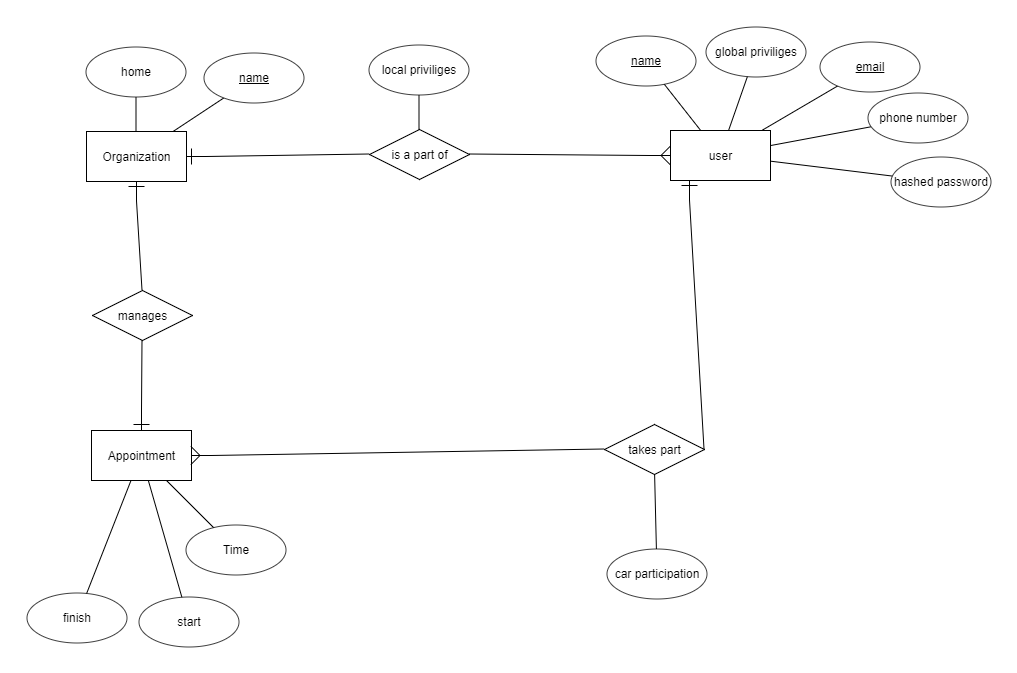
\includegraphics[width=\textwidth]{ER_Diagram.png}
\caption{ER-Diagram für Interne Mitfahrgelegenheit}
\end{figure}

\end{document}
